\documentclass[12pt, a4paper]{article}
% Packages: 
\usepackage[utf8]{inputenc}
\usepackage[T1]{fontenc}
\usepackage[polish]{babel}
\usepackage[utf8]{inputenc}
\usepackage{lmodern}
\usepackage{graphicx}
\usepackage{indentfirst}
\usepackage{fancyhdr}
%------------------------------------
% Style config etc.:
\selectlanguage{polish}
\brokenpenalty=1000
\clubpenalty=1000
\widowpenalty=1000    
\pagestyle{fancy}
\fancyhead{}
\fancyfoot{}
\rfoot{\thepage}
\lfoot{}
\lhead{}
\rhead{}
\renewcommand{\headrulewidth}{1pt}
\renewcommand{\footrulewidth}{1pt}

\title{Konfiguracja serwera DHCPv4 oraz serwera DHCPv6 w prostej podsieci, wraz z przekierowaniem rozgłoszeniowych zapytań DHCP.}
\author{Marian Dorosz}
\date{}

\begin{document}

\maketitle
\newpage

\tableofcontents
\newpage

\listoffigures
\newpage

\section{Konfiguracja serwera DHCPv4}
%Serwer DHCPv4 to komputer z zainstalowanym systemem Windows Server 2008. 
    \subsection{Schemat podsieci wraz z adresacją IPv4.}
        \begin{figure}[!h]
            \centering
            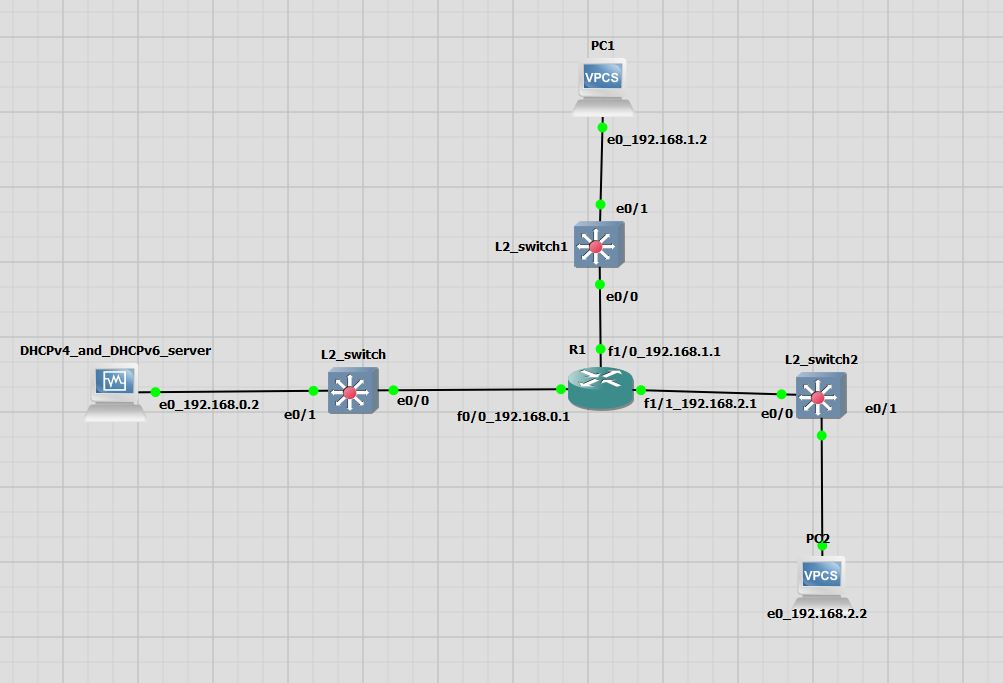
\includegraphics[scale = 0.456]{podsiec_dhcpv4.JPG}
            \caption{Urządzenia w podsieci wraz z ich adresami}
            \label{fig:dhcpv4}
        \end{figure}
        Widoczny na rysunku serwer DHCP, to komputer z zainstalowanym systemem Windows Server 2008. Serwer ten posiada zainstalowaną rolę DHCP i w ramach tej roli zostały wydzielone dwa zakresy, w oparciu o które serwer przydziela hostom adresy.
        \begin{itemize}
            \item Zakres pierwszy: 192.168.1.2 - 192.168.1.254,
            \item zakres drugi: 192.168.2.2 - 192.168.2.254\footnote{Oba te zakresy dotyczą podsieci o masce 255.255.255.0.}.
        \end{itemize}
    \subsection{Konfiguracja rutera}
        Ruter R1 jest skonfigurowany tak, aby działał jako \textit{relay agent}, czyli urządzenie, które przesyła rozgłoszeniowe zapytania DHCP przez sieć, tak aby mogły trafić do serwera. Po otrzymaniu zapytania DHCP ruter generuje nowy pakiet DHCP, w oparciu o pakiet, który wcześniej otrzymał. W tym nowym pakiecie umieszcza on nowy adres IP (\textit{helper address}). Adres ten to adres serwera DHCP, na który ma trafić przesłany dalej pakiet DHCP. Istnieje również możliwość, że w nowym pakiecie ruter dopisze parametry tzw. opcji 82. Są to dodatkowe parametry, które mogą zostać przesłane do serwera tak, aby ten mógł w ich oparciu podjąć dodatkowe decyzje odnośnie adresacji hosta.
%-------------------------------------------------------------------------------------
\section{Konfiguracja serwera DHCPv6}
%Serwer DHCPv4 to komputer z zainstalowanym systemem Windows Server 2008. 
    \subsection{Schemat podsieci wraz z adresacją IPv6.}
        \begin{figure}[!h]
            \centering
            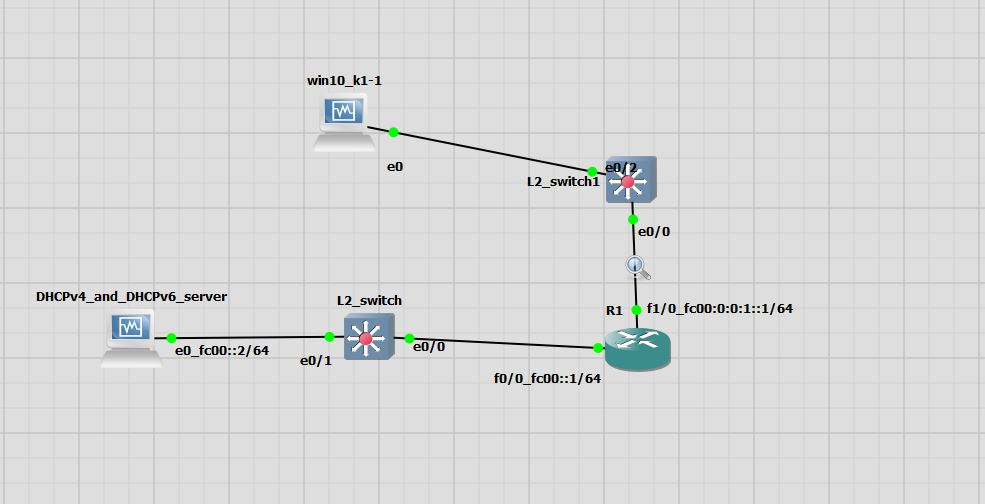
\includegraphics[scale = 0.456]{podsiec_dhcpv6.JPG}
            \caption{Urządzenia w podsieci wraz z ich adresami}
            \label{fig:dhcpv6}
        \end{figure}
        Widoczny na rysunku serwer DHCP, to komputer z zainstalowanym systemem Windows Server 2008. Serwer ten posiada zainstalowaną rolę DHCP i w ramach tej roli zostały wydzielony jeden zakres adresów IPv6: \textbf{fc00:0:0:1::3 - fc00::1:ffff:ffff:ffff:ffff}
    \subsection{Konfiguracja rutera}
        Ruter R1 jest skonfigurowany tak, aby działał jako \textit{relay agent}, czyli urządzenie, które przesyła rozgłoszeniowe zapytania DHCP przez sieć, tak aby mogły trafić do serwera. Ruter informuje urządzenia o fakcie, że w sieci jest obecny serwer DHCPv6 i to nie on przydziela hostom dane adresowe, dlatego komputery aby uzyskać adres IPv6 wysyłają zapytanie DHCP, które ruter przesyła do podsieci, w której jest serwer.
\end{document}
